% ABLS - term-long paper

\documentclass{sig-alternate}

\usepackage{url}
\usepackage{color}
\usepackage{enumerate}
\usepackage{balance}
\usepackage{verbatim}
\usepackage{enumitem}
\usepackage[table]{xcolor}
\usepackage{multicol,multirow}
\usepackage{subfig}
\usepackage{dcolumn}
\usepackage{palatino}
\usepackage{bbm}
\usepackage{url}
\usepackage{verbatim}
\usepackage{algorithm}
\usepackage[noend]{algorithmic}
\usepackage{fancybox, fancyvrb}
\usepackage{listings}

\permission{}
\CopyrightYear{2012}
%\crdata{0-00000-00-0/00/00}
\begin{document}

\title{ABLS - An Attribute Based Logging System for the Cloud}
\numberofauthors{1}
\author{
\alignauthor{
Christopher A. Wood \\
Department of Computer Science \\
{\tt caw4567@rit.edu}
}}
\date{\today}
\maketitle
\begin{abstract}
User-based non-repudiation is an increasingly important property of cloud-based applica-tions. It provides irrefutable evidence that ties system behavior to specific users, thus enabling strict enforcement of organizational security policies. System logs are typically used as the basis for this property. Thus, the effectiveness of system audits based on log files reduces to the problem of maintaining the integrity and confidentiality of log files. In this project, we study the problem of building secure log files. We investigate the benefits of ciphertext-policy attribute-based encryption (CP-ABE) to solve a variety of log design issues. In addition, we also present the architecture and a preliminary analysis for a proof-of-concept system that fulfills the confidentiality and integrity requirements for a secure log.
\end{abstract}

\section{Introduction}
User-based non-repudiation is a system security property that provides indisputable evidence that links
specific actions to individual users (or entities) that trigger such actions. Cryptographically speaking, non-repudiation requires that the integrity and 
origin of all data should be provable. In essence, this enables system audits to be conducted that can
identify data misuse (and thus, potential security policy violations) by comparing the sources of system events
with all entities authorized to invoke these events. Therefore, treating non-repudiation as a required system 
quality attribute in the architecture is likely to become a common trend in the commercial, 
government, and even more specifically, the health-care domain.

System audits typically use log files to determine the cause and effect of events that took 
place during the system's lifetime. In order to provide accurate information for non-repudiation purposes,
it is often necessary to place some amount user-sensitive data in these log files that can be used
to trace data back to its origin. As such, logs of events generated by a client that is being served must
maintain data confidentiality and integrity should the system be compromised. These goals are commonly achieved
using a combination of encryption and signature techniques \cite{Ma2008-FssAgg}. However, traditional approaches to
encryption and signature generation and verification are becoming less effective in the context of cloud
applications. Furthermore, naive approaches to log security that are based on tamper-resistant hardware and 
maintaining continuous secure communication channels between a log aggregator and end user are no longer useful in 
the context of cloud-based applications \cite{Schneier1999-Secure}. 

Symmetric-key and public-key encryption of log entries are very common confidentiality techniques 
proposed in the literature. However, in cloud-based applications, these schemes are becoming less useful.
There is a need for a robust access control mechanism that enables dynamic user addition and revocation
with minimal overhead (i.e. re-encrypting a subset of the log database should be avoided). Both symmetric- and 
public-key cryptosystems lack in that access policies must be tied directly to keys used for
encryption and decryption. If the access policy for a set of log messages needs to be changed, then both the keys used to
encrypt and decrypt such log entries will need to be regenerated and distributed, and the entries must also
be re-encrypted. Both of these tasks can be very expensive. 

In addition, symmetric-key cryptosystems require keys to be shared among users who need access to the 
same set of logs, which requires a secure and comprehensive key management and distribution policy. 
From a storage perspective, public-key cryptosystems (e.g. RSA and ElGamal) suffer from the extra data transfer and 
storage requirements for large cryptographic keys and certificates. There may be insufficient resources 
to maintain a public-key infrastructure (PKI) for managing keys and digital certificates for all users. 

In terms of log file integrity, aggregate signature schemes that support forward secrecy through the use of 
symmetric- and public-key cryptosystems are also becoming outdated \cite{Yavuz2009-BAF}. Symmetric-key schemes may promote
high computational efficiency for signature generation, but they do not directly support public verifiability for 
administrators and auditors. This means that robust key distribution schemes or the introduction of a trusted third party (TTP) are needed to ensure all required parties can access the necessary log information. Such schemes also 
suffer from high storage requirements and communication overhead. Public-key schemes have similar issues, 
as the increased key size leads to even larger storage requirements and less computational efficiency. 

Collectively, we see that a balance between encryption and signature generation and verification performance is
needed to support the unique scalability and resource usage requirements for cloud-based applications.
Attribute-based encryption (ABE), a new cryptographic scheme that uses user attributes (or roles, in certain 
circumstances) to maintain the confidentiality of user-sensitive data, has an appealing application
to logging systems maintained in the cloud and is capable of satisfying the aforementioned confidentiality 
requirements. In addition, authenticated hash-chains have been shown to be effective at enforcing log file integrity
in numerous logging schemes  \cite{Schneier1999-Secure}. 

ABLS, an attribute-based logging system that supports ciphertext-policy attribute-based encryption (CP-ABE) \cite{Bethencourt2007-CPABE} 
and authenticated hash-chain constructions for log file confidentiality and integrity, respectively, was recently designed and implemented
by the primary author.  The preliminary ABLS architecture and design was weak with regards to the 
scalability of encryption operations under heavy traffic loads,
the relational database schema to store log-data and other sensitive information, and the interactions 
with database servers. To address these issues,
we propose a set of extensions that modify ABLS in the following ways:
\begin{enumerate}
	\item The CP-ABE encryption scheme will be replaced with a hybrid cryptosystem in which the Advanced
	Encryption Standard (AES), the standardized symmetric-key encryption algorithm, is used to encrypt user
	session data by a key that is protected with CP-ABE encryption. In the event that a user generates log messages
	with varying sensitivity levels during a single session, multiple symmetric keys will be produced to maintain
	the confidentiality of information in different security classes.
	\item The relational database storage scheme will either be changed to include a masking column in the appropriate
	log table to hide user identities or replaced entirely with a document- or object-based database. Both of these
	modern database systems are similar in semantics (if documents are conceptually treated as serialized objects),
	so a product and literature survey will be conducted prior to selecting an adequate replacement that satisfies
	the necessary security and performance requirements. Though, based on preferences and architectural experience,
	a document-based database such as MongoDB will be the likely candidate. Also, since the ABLS architecture is highly
	structured around a relational schema to store data, this change will require modifications made in the logging, attribute authority, 
	and auditing modules in order to maintain functional correctness. 
	\item Database security mechanisms, including fine-grained access policies for protected databases and encryption of data-in-transit, 
	will be implemented. This is particularly
	important for the databases that store cryptographic keys. Also, since preference is given to document-based databases such as MongoDB,
	third-party services such as zNcrypt (provided by Gazzang) that are specifically tailored to this DBMS will likely be used to enforce 
	access control to sensitive databases.
	\item The auditing module will be extended to include automated audits of database operations, including changes
	to the database structure and both successful and unsuccessful client connections with the database. Currently,
	the auditing module is only designed (and partially implemented) to support strategy-based audits on database contents. However,
	in this type of application, database performance and security are just as critical. Thus, with this change, there will be two audit 
	techniques that can roughly be equated to data and policy inspections, both of which will only be accessible to users with the
	appropriate privileges. This access control will be likely be enforced using username and password credentials.
\end{enumerate}

Altogether, the security features of database authentication, encryption, and auditing will be further expanded upon
in the existing ABLS architecture. With these changes, we will then re-evaluate the ABLS at an architectural, security, 
and performance perspective to determine its usefulness in cloud-based settings. 

\section{Log Design}
In this section we present our log generation and verification schemes.
They are influenced by past work done by Schneier et al \cite{Schneier1999-Secure},
Bellare et al. \cite{Bellare1997-ForwardIntegrity}, Ma et al. \cite{Ma2008-FssAgg},
and Yavuz et al. \cite{Yavuz2009-BAF}. 

\subsection{Log Construction}
\label{sec:LogConstruction}

Log integrity is achieved through hash chains and message-authentication codes. 
Each log entry is a five-tuple element that contains the generating source
information, the encrypted payload of the entry, a hash digest that provides
a link between the current and previous hash chain entries, and an authentication tag for this digest. In the proof-of-concept
system implementation, Keccak is used as the standalone hash function $H$
and the $HMAC$ function is built using $SHA$-$512$. 
Formally, each log entry $L_i$ is built using the following protocol (as depicted in Figure \ref{fig:hashChain}):
\begin{align*}
X_i = & H(X_{i - 1}, E_{SK}(D_i)) \\ % rationale: need to link this entry to previous for chaining
Y_i = & HMAC_{EpK_{j}}(X_i, Ep_{j}) \\ % rationale: for epoch-key based: can keep in logger memory and then commit on epoch cycle (helps against wiretapping attacks and load balancing)
L_i = & (U_{ID}, S_{ID}, E_{SK}(D_i), X_i, Y_i) % rationale for u/s: searhability
\end{align*}

\begin{figure*}[ht!]
  \centering
  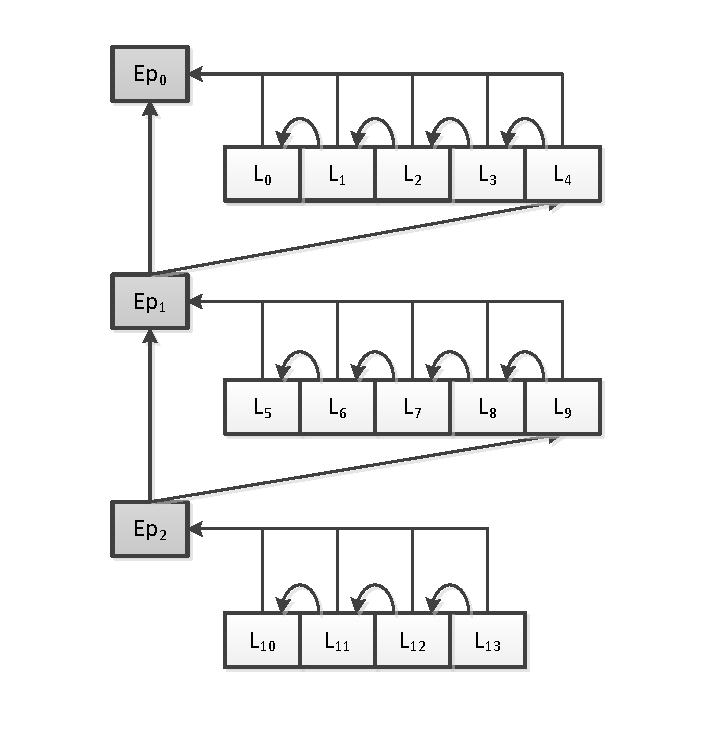
\includegraphics[scale=0.8]{images/hashchain.pdf} \\
\caption{A visual depiction of the hash chain construction scheme. In this case, the epoch window is $5$ log entries, as shown by the epoch
cycle after $5$ consecutive log entries.}
\label{fig:hashChain}
\end{figure*}

In this scheme the $X_i$ elements are used to link together consecutive entries in 
the hash chain. Similarly, the $Y_i$ elements are used to provide authentication 
for the $X_i$ element using an authentication tag that is computed from $X_i$ and the 
previous epoch digest $Ep_{j - 1}$. 

In this context, an epoch $Ep_j$ simply corresponds to a fixed-size set of log entries that
are being processed (i.e. an epoch window). For example, if the epoch size is $n$ entries, then the 
log generation scheme will cycle after $n$ log entries have been constructed and begin working on a new set of log entries. After a cycle is completed, a context block
for the most recent epoch is created and inserted into an epoch chain (similar to the log chain). These log generation cycles create frames (or windows) in the entire log chain in which the 
scheme generates log entries using a single epoch block and key $Ep_{j}$ and $EpK_j$, respectively. 
More specifically, $Y_i$ is the authentication tag that is built using only the entries within the current epoch window.

%TODO: forward-secrecy guarantees... compare to aggregate signatures (we store each hash chain and the entire thing altogether)

%In order to provide computationally efficient means of generating the 
%authentication tag for the log chain, log generation is divided into epochs of
%client-defined sizes. The selection criteria for this epoch size is 
%discussed in more detail later, but should generally be based
%on the frequency of traffic that is generated by the host application. 

Context blocks for epoch windows are stored in the same way as log chains.
Each epoch chain entry $Ep_j$ is built as follows:
\begin{align*}
Ep_j = & HMAC_{EpK_{j}}(Ep_{j - 1}, L_{l}) \\
Ep_0 = & HMAC_{EpK_{0}}(0)
\end{align*}
In this context, $L_{l}$ is the last log chain entry for the previous epoch $Ep_{j - 1}$.
Thus, each epoch chain entry maintains the integrity of the log chain at each epoch cycle
by linking the most recent log chain entry to the previous epoch context block.
The key $EpK_{j}$ that is used to compute the $Y_i$ authentication tag is
based on the current epoch $Ep_j$, and only evolves when the epoch window cycles. 
This update is done with a pseudorandom function $H$ (which,
in our case, is simply the Keccak hash function), and is defined as follows:
\begin{align*}
EpK_{j + 1} = H(EpK_{j}) \\
\end{align*}
The initial epoch key $EpK_0$ is a secret that is initialized when a session
is started. Corruption of this key can enable a determined attacker to reconstruct
the log chain and epoch chain without detection. Without this information, however,
such modifications are always detectable. We refer to Section \ref{sec:security} for
a more detailed description of this issue.

Finally, as a third layer of integrity, a single digest for the entire log $T_i$
chain is stored as the log chain is iteratively constructed. Formally, $T_i$ is
built as follows:
\begin{align*}
T_i = & HMAC_{T_{K_{i}}}(L_{i}, T_{i - 1}) \\
T_0 = & HMAC_{T_{K_{0}}}(L_{i}, 1) %caw: this needs to change in the code. current code does not do it this way.
\end{align*}
The secret key $T_{K_{0}}$ for the entire log chain is another secret that is
initialized when the session is started. Similar to the epoch key, it is evolved
with a pseudorandom function $H$ as follows:
\begin{align*}
T_{K_{i + 1}} = H(T_{K_{i}})
\end{align*}

A visual representation of this protocol is shown in Figure \ref{fig:tagChain}. It is
important to note that a chain of $T_i$ elements is not maintained. Instead, only the
most recent element is persisted to the database. This is critical to prevent
truncation attacks.

\begin{figure*}[ht!]
  \centering
  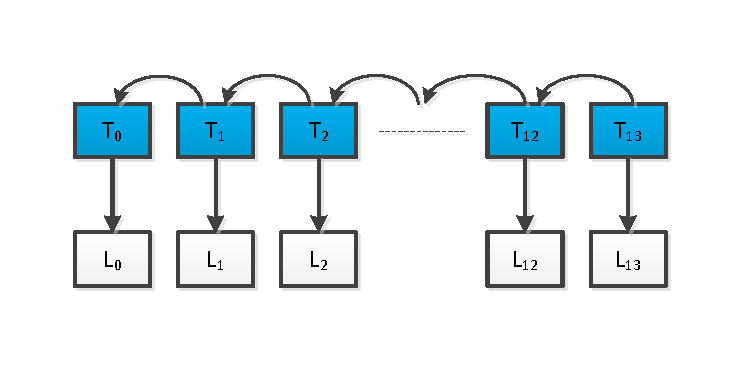
\includegraphics[scale=0.8]{images/tagchain.pdf} \\
\caption{A visual depiction of the protocol used to build the log chain authentication tag.}
\label{fig:tagChain}
\end{figure*}

\subsection{Log Generation Rationale}
The construction of each log entry satisfies the following properties:
\begin{enumerate}
	\item Each log entry payload is encrypted and only viewable by those with the appropriate attributes.
	\item The integrity of the log chain is ensured through the links generated by $X_i$ elements, which are verifiable by the $Y_i$ authentication tags.
	\item The integrity of the entire log chain is guaranteed with the $T_i$ element. This protects the log chain against truncation attacks.
	\item The epoch-based log generation enables the logger to control the frequency of data
	sent to the log server, which helps with load balancing and protects against wiretapping attacks.
	\item The epoch window is assumed to be a fixed (constant) size, and thus it requires $\mathcal{O}(1)$ time to verify. The log chain can be verified in $\mathcal{O}(n)$ time, where $n$ is the length of the log chain. These results are discussed in Section \ref{log:ComputationalComplexity}.
	\item There are three different modes of verification that can be performed (weak, normal, and strongest). These modes are described in Section \ref{log:VerificationModes}.
	\item The log is searchable by the user identity and session numbers, which leads to very fine-grained database queries. 
\end{enumerate}

\begin{comment}
\subsection{Searchability}
Based on the definitions provided in Section \ref{sec:LogConstruction}, it is easy to 
see that log searchability is done by querying the database with known user identities and optional session 
identifiers. This was a tradeoff that we made to support reasonable auditing performance. 
It has been shown that in some application domains the presence of any relevant information
pertaining to users is a violation of security policies. However, since the entire entry payload
is kept confidential to unauthorized users through encryption, we do not anticipate the presence 
of this information causing many problems. 

The database schema for our logging system is shown in Figure \ref{fig:schema}. We emphasize that, 
if the log server were compromised, the only information that a determined attacker could retrieve from
the log database is a collection of user identities, which do not directly correspond to ``real'' user
identities (i.e. database user identities are GUIDs that are generated whenever a user account is created
by the host application). 
\end{comment}

\section{Implementation}
In order to test both the correctness and performance of ABLS, a proof-of-concept system has been
developed. In this section we provide the design and rationale for the prototype architecture.

\subsection{Deployment}
\label{sec:deployment}
ABLS is designed to be a centralized logging system backed by a set of distributed databases. A context
diagram for the ABLS deployment scheme is shown in Figure \ref{fig:deployment}, and a more detailed
depiction of the flow of data between application and database servers is shown in Figure \ref{fig:design}.

%TODO: rough deployment diagram for ABLS (different from architecture diagram)

%\begin{figure*}[htb!]
%\label{fig:design}
%\begin{center}
%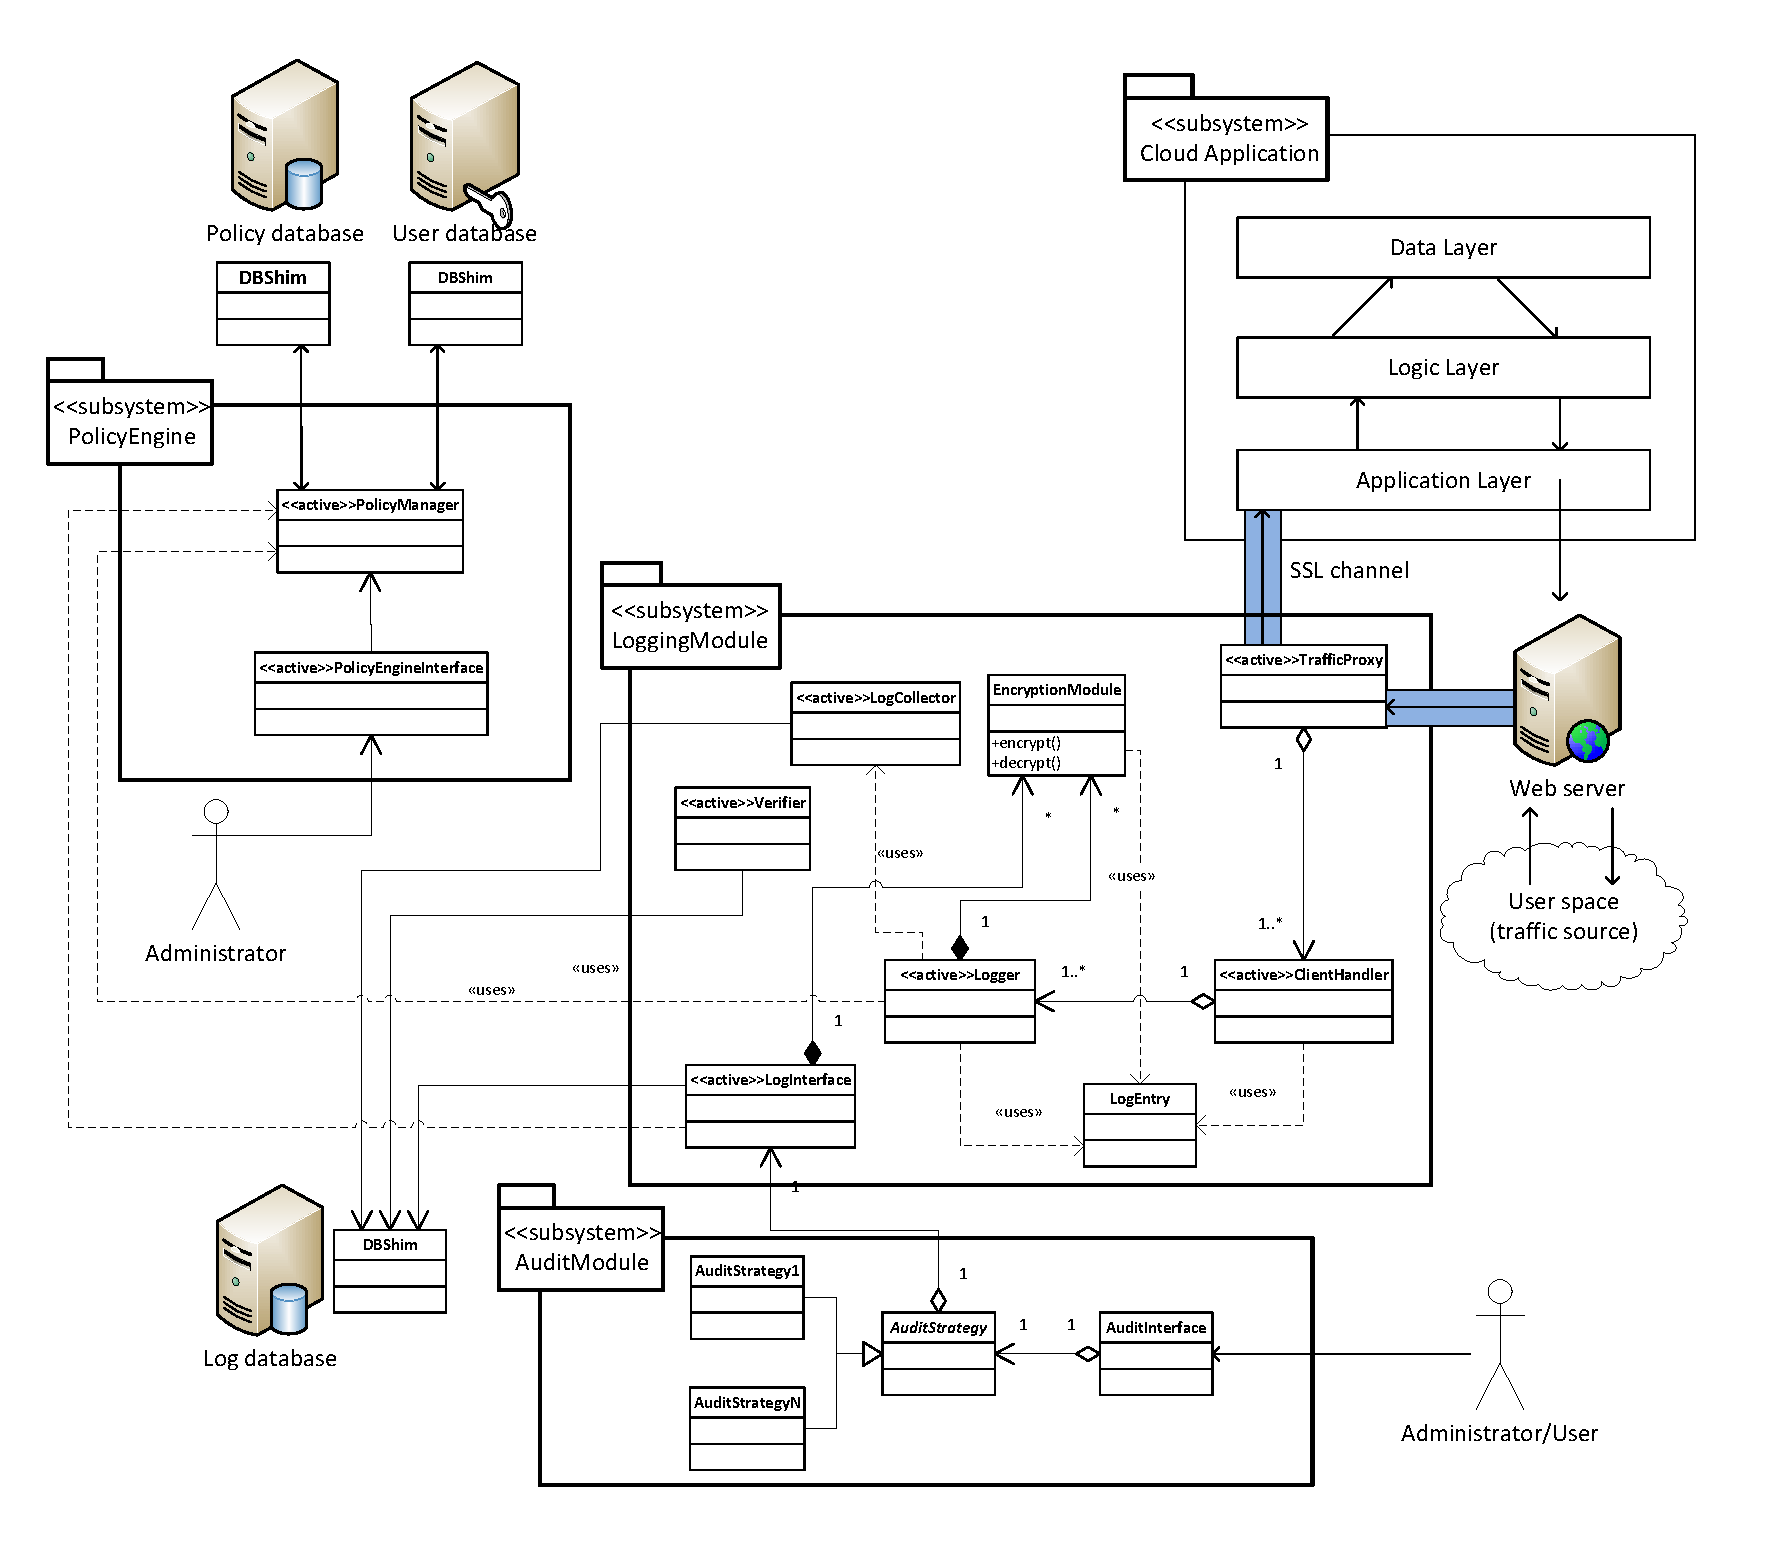
\includegraphics[width=7in]{images/design.pdf}
%\caption{The deployment diagram for ABLS.}
%\end{center}
%\end{figure*}

Based on the purpose of each piece of database used in the log, it is best to physically separate databases
that store data of different security classes rather than rely on MAC with polyinstantiation. Of course, access control
and authentication mechanisms for all database servers is enforced at the operating system level, thus
prohibiting immediate access to all unauthorized users other than the {\tt LoggingModule} and {\tt PolicyEngine} 
processes. 

In the current ABLS prototype, all database servers are separated as individual SQLite database files. Once
the deployment platform is selected and properly configured, these will be replaced with instances of MySQL 
databases running on separate servers.

\subsection{Key Management}
\label{sec:keyMgmt}
In order to increase the performance of log entry encryption during a given user session, symmetric-key encryption
using AES-256 is chosen to encrypt all log entry messages. The symmetric key is then encrypted using the CP-ABE
scheme. This design enhancement enables increased improvement without sacrificing the level of confidentiality 
granularity that is needed for each log entry. 

The basic algorithm for encrypting a log entry is shown in Algorithm \ref{alg:encrypt}. Once encrypted, the cipher text
is stored as specified in Section \ref{sec:LogConstruction}.

\begin{algorithm}[ht!] %[htb]
\caption{Log entry encryption} \label{alg:encrypt}
\begin{algorithmic}[1]
\REQUIRE{An unencrypted log entry $L_i$ for session $S_j$ of user $U_k$}
% \ENSURE{The number of all minimum $(s,t)$-cuts of $G$}

% I decided not to list the input/output in this case, so that's why the above two lines are commented out
\STATE{Let $P$ be the access control policy for the message of $L_i$, as determined by the {\tt PolicyManager}}
\IF{The symmetric key $K$ for $(U_k, S_j)$ has not been generated for $P$}
	\STATE{Generate $K$ and encrypt it (with the CP-ABE encryption module) using $P$}
	\STATE{Persist $K$ to the key database}
\ENDIF
\STATE{Encrypt $L_i$ with AES-256 using $K$, yielding $E(L_i, K)$}
\STATE{Persist $(L_i, K)$ to the log database}
\end{algorithmic}
\end{algorithm}

\subsection{Database Design}
\label{sec:databaseDesign}
As shown in section \ref{sec:deployment}, there are four main databases that must be maintained by ABLS:
the log, key, user, and policy database. The log database maintains the all information in the log chain for every 
single user and session pair. The key database stores the cryptographic keys that were used to construct
such log chains. The user and policy databases store user information and policy rules for ABLS, respectively. 
In the current prototype of ABLS, the policy database is not used externally. All event rules are hard-coded into
the {\tt PolicyEngine}. 

In order to link the entries in the log tables to their corresponding verification and encryption keys in the key database,
common user and session IDs are used (though not as the primary key for the tables since they do not satisfy
the uniqueness property). However, because such the storage of such user and session information in plaintext
may lead to violation of user privacy, they are deterministically masked before being stored in the database. 

This masking procedure works by encrypting the user and session attributes with a symmetric key generated
by the logger's master key salted by the user's unique identifier. Specifically, the encrypted user and session IDs, 
$[U_i]$ and $[S_j]$, are generated as follows.
\begin{align*}
[U_i] = E(M_k || H(U_i), U_i) \\
[S_j] = E(M_k || H(U_i), S_j) \\
\end{align*}

TODO: discuss how the salt changes for each table so attackers can't link things together...

%\section{Auditing}
%TODO: Initial audit design implemented

\newpage

\section{Completed Work}
For Phase 1 of the project, I focused mainly on fixing some of the design and implementation flaws in my previous 
prototype, redesigning the database to support the new symmetric key management scheme and data 
partitioning for different security classes, specifying the deployment scheme, and improving the quality test
of my internal unit tests and the functionality of the test driver program. The specifics of each of these improvements is
outlined in the following sections.

\subsection{Symmetric Key Management}
As described in Section \ref{sec:keyMgmt}, the process of encryption log messages was changed to use symmetric-key
encryption instead of CP-ABE due to the added performance improvement. Pairing-based cryptography is computationally
expensive, and under the assumption that ABLS might be subject to very heavy traffic loads at any particular time, the 
overhead of encrypting data to be stored in the database should be as minimal as possible. Therefore, each unique
policy that is needed to encrypt a log message is associated with a symmetric key, which is in turn encrypted and 
serialized using CP-ABE. The Charm crypto package allows all cryptographic objects (which tend to be nested
Python dictionaries and other complicated data structures) to be serialized to byte representations for database 
persistence. 

Also, in order to improve the performance of the logger, the per-policy symmetric keys for a user session are kept
in memory until the session has been closed. This avoids the need for the logger to query the database for the key 
when a new piece of data to be inserted into the log. 

\subsection{Relational Database Design}
The relational database design was modified in order to support the new symmetric key management scheme and provide 
enhanced security for the stored data. In particular, rather than storing the cryptographic keys in the same database as the
log information, these two databases are now segregated and are expected to be deployed on different database servers.
By hardening both databases, a malicious attacker would need to circumvent the access control mechanisms protecting
two physically disjoint databases, rather than just one. 

In addition, to better support audits that use the log database, a timestamp field was added to each table as a required
attribute. Not only does such information capture the exact timing of critical system events, it acts as a protection
mechanism in the event that log messages are inserted into the database out of order. Also, it is important to note that
each and every timestamp for a log message is generated as soon as the {\tt ClientHandler} reads the data from
its open socket. This is done to provide the most accurate timing information.

%Redesigned the relational database model to account for the different security classes among data that is used by ABLS. This resulted in a physical separation of database servers.
%TODO: added times, separated the database tables, optimized data types for columns to match what's stored

\subsection{Database Column Masking}
The initial implementation of the database masking procedure, which is outlined in Section \ref{sec:databaseDesign}
was started in this phase of the project. Currently, only the ability for the logger to store the encrypted user and session IDs 
is supported. The verifiers have yet to be updated to use this encrypted data to perform the strong verification check. This 
will finished in the next phase of the project.

\subsection{Bootstrapping, Test Enhancement, and Deployment}
In order to streamline the test and deployment phases of development, a bootstrap script was implemented to configure
new (empty) versions of the local SQLite databases. The main executable script (main.py) was also modified to support
debug and production modes of operation, in which the debug mode clears the contents of every database and
then proceeds to insert false user data into the users table to begin the logging process. The test driver program,
TrafficProxyDriver.py, is then modified accordingly to use the default data contained within the database. With these
changes, the typical process to start the ABLS system is as follows.

\begin{enumerate}
	\item 
\end{enumerate}

Aside for the initialization code, the test driver program now includes a more robust suite of tests to simulate varying traffic 
loads. The user interface of this program was also improved so as to aid the developers in interacting with the ABLS 
prototype at runtime. Given the difficulty of testing this distributed system at runtime, creating a more sophisticated
test driver was crucial to the development process that enabled smoke tests to be run with minimal effort.

However, despite the increased complexity of the test driver, it does not, nor will it ever, support the ability to acquire 
diagnostic information from the ABLS runtime. This information is logged by the ABLS runtime to the appropriate log 
file, and the administrators for the ABLS system can check this information at their discretion.

\subsection{Literature Survey}
TODO: brief discussion of the literature survey here

\section{Future Work}
For the remainder of the project I plan to finish up the partially completed work introduced in the previous section and 
focus on the auditing aspect of ABLS. Auditing will be supported both manually and automatically through
a robust log query interface, which places the ABLS runtime in the role of the reference monitor, and automated
strategy-driven tasks run within the context of the ABLS runtime, respectively. The following sections expand upon all
of these action items in more detail.

% expand on this - it should fill 3/4 of a page

\subsection{Complete Database Masking}
- encrypting and masking user identity attributes in all of the databases

\subsection{Log Collection}
TODO: started on the log collection actors

\subsection{Log Querying}
- design and implement an easy API for querying information from the log (and only the log) table that checks user authentication privileges first - the logger is the reference monitor to the outside world

- variety of selection functions in which the user can specify the user ID or user and session ID, all data that comes back
is verified using strong verification, contents of the log messages are filtered depending on their policy (only if the policy matches the client's attributes will the results be returned)

- outline process of querying (client is authenticated with username/password, attributes are generated, database is queried using encrypted data, results are filtered based on policy, and result is returned)

\subsection{Audit Strategy Design}
- auditing design and implementation (define automated worker tasks that use pre-defined strategies for
auditing (search by userID) or whatnot that can be triggered by any web application set in front of ABLS - 
making it easy for auditors to start their own automated audits). 

\begin{comment}
\begin{table}
\centering
\caption{Feelings about Issues}
\begin{tabular}{|l|r|l|} \hline
Flavor&Percentage&Comments\\ \hline
Issue 1 &  10\% & Loved it a lot\\ \hline
Issue 2 &  20\% & Disliked it immensely\\ \hline
Issue 3 &  30\% & Didn't care one bit\\ \hline
Issue 4 &  40\% & Duh?\\ \hline
\end{tabular}
\end{table}

\begin{figure}[htb]
\label{sample graphic}
\begin{center}
\includegraphics[width=1.5in]{fly.jpg}
\caption{A sample black \& white graphic (JPG).}
\end{center}
\end{figure}
\end{comment}

\bibliographystyle{abbrv}
\bibliography{../abls}
% You must have a proper ".bib" file
%  and remember to run:
% latex bibtex latex latex
% to resolve all references
\balance
\end{document}
